\Exercise[number={10}]
In an experiment, real and positive quantities \(x\) are measured, described
by an exponential distribution:
\[
    p(x|\lambda) \propto \lambda^{-x}
\]
where \(\lambda>0\) is a parameter. \\
a. Determine the normalization factor \(K\). [Hint: should be
\(K\int_0^{+\infty}\lambda^{-x}\,dx = 1\)
] \\
b. Given a \(x\), analyze the function \(L(\lambda)=p(x|\lambda)\) and
display it in a Cartesian graph. \\
c. Given \(N\) independent measures \(\bigl\{ x_n, n=1,...,N \bigr\}\),
derive a maximum likelihood estimator for \(\lambda\).

\Answer[number={10}]
a. To find the normalization term \(K\), the integral between 0 and \(+\infty\) is to
be calculated:
\begin{align*}
    \int_{0}^{+\infty}Kp(x|\lambda)\,dx = 1
    \Rightarrow
    K\int_{0}^{+\infty}\lambda^{-x}\,dx
    =
    K\biggl[\frac{\lambda^{-x}}{\log{\lambda}}\biggr]_{0}^{+\infty}
\end{align*}
Notice that the integral is undefined as long as \(\lambda \le 1\), thus
a new condition is to be set, in particular \(\lambda > 1\), leading
to the integral expression below:
\begin{align*}
    \int_{1}^{+\infty}Kp(x|\lambda)\,dx = 1
    \Rightarrow
    K\int_{1}^{+\infty}\lambda^{-x}\,dx
    =
    K\biggl[\frac{\lambda^{-x}}{\log{\lambda}}\biggr]_{1}^{+\infty}
    =
    \frac{K}{\log{\lambda}}=1
    \Rightarrow
    K=\log{\lambda}
\end{align*}
b. The likelihood \(L(\lambda|x)=\log{(\lambda)}\lambda^{-x}\). Given the
preivous considerations, the domain is \(\lambda>1\) and the likelihood
has a positive sign in the whole domain. The asymptotes are computed as:
\begin{align*}
    \lim_{\lambda\to{1^+}}\log{(\lambda)}\lambda^{-x} = 0 \\
    \lim_{\lambda\to{+\infty}}\log{(\lambda)}\lambda^{-x} = 0
\end{align*}
Let's compute the derivative of \(L(\lambda)\) and study its sign:
\begin{align*}
    \frac{d\,L(\lambda)}{d\,\lambda}
    =
    \frac{d\,\log{(\lambda)}\lambda^{-x}}{d\,\lambda}
    =
    \frac{\lambda^{-x}}{\lambda}+\log{(\lambda)}(-x)\lambda^{-(x+1)}
    =
    \lambda^{-(x+1)}\bigl[1-x\log{\lambda}\bigr]
\end{align*}
\begin{align*}
    \cancel{\lambda^{-(x+1)}}\bigl[1-x\log{\lambda}\bigr] > 0
    \Longleftrightarrow
    1-x\log{\lambda} > 0
    \Longleftrightarrow
    \log{\lambda} < \frac{1}{x}
    \Longleftrightarrow
    \lambda < e^{\frac{1}{x}}
\end{align*}
Therefore, \(\lambda = e^{\frac{1}{x}}\) is the global maximum for the
likelihood function in the given domain \(\lambda>1\). \\
The likelihood as function of \(\lambda\) exhibits the following plot:
\begin{figure}[H]
    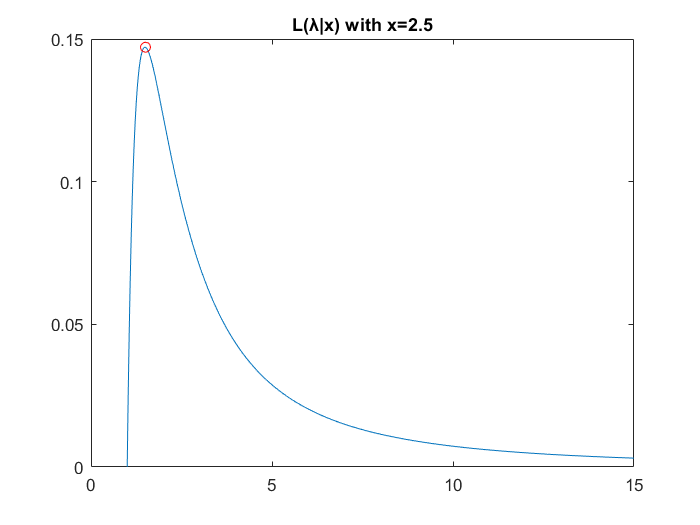
\includegraphics[scale=0.65]{B_10}
    \centering
\end{figure}
c. Let's define a dataset \(X=\{x_n, n=1,...,N\}\), then the likelihood
can be written as \(L(\lambda|X)=\prod_{i=1}^{N}\log{(\lambda)}\lambda^{-x_i}\).
Thus, the log-likelihood is:
\begin{align*}
    \log{L(\lambda|X)}=\sum_{i=1}^{N}\log{(\log{\lambda})}-\sum_{i=1}^{N}x_i \log{\lambda}
    =
    N\log{(\log{\lambda})} - \log{\lambda}\sum_{i=1}^{N}x_i
\end{align*}
By taking the derivative of the log-likelihood and setting it to zero, the
maximum likelihood estimator \(\hat{\lambda}\) can be obtained:
\begin{align*}
    \frac{\partial{\log{L(\lambda|X)}}}{\partial{\lambda}}=0
    &\Rightarrow
    \frac{N}{\log{\lambda}}\frac{1}{\lambda}-\frac{1}{\lambda}\sum_{i=1}^{N}x_i=0 \\
    &\Rightarrow
    \frac{1}{\lambda}\biggl[\frac{N}{\log{\lambda}} - \sum_{i=1}^{N}x_i\biggr]=0 \\
    &\Rightarrow
    \hat{\lambda_1}\to +\infty,
    \quad\quad
    \frac{N}{\sum_{i=1}^{N}} = \log{\lambda} \Rightarrow \hat{\lambda_2}=e^{\frac{N}{\sum_{i=1}^{N}x_i}}=e^{\frac{1}{mean(X)}}
\end{align*}
Notice how \(\hat{\lambda_2}\) has a form consistent with the global maximum
obtained before for a single value \(x\).